\chapter{Minimum Spanning Tree}

Sebuah Spanning Tree merupakan sebuah potongan graph (subgraph) satu arah yang menghubungkan semua vertex menjadi sebuah tree. Sebuah graph dapat memiliki beberapa Spanning Tree sekaligus. Gambar~\ref{fig:spanning-tree-intro} menunjukkan contoh beberapa Spanning Tree dari sebuah graph.

\begin{figure}
    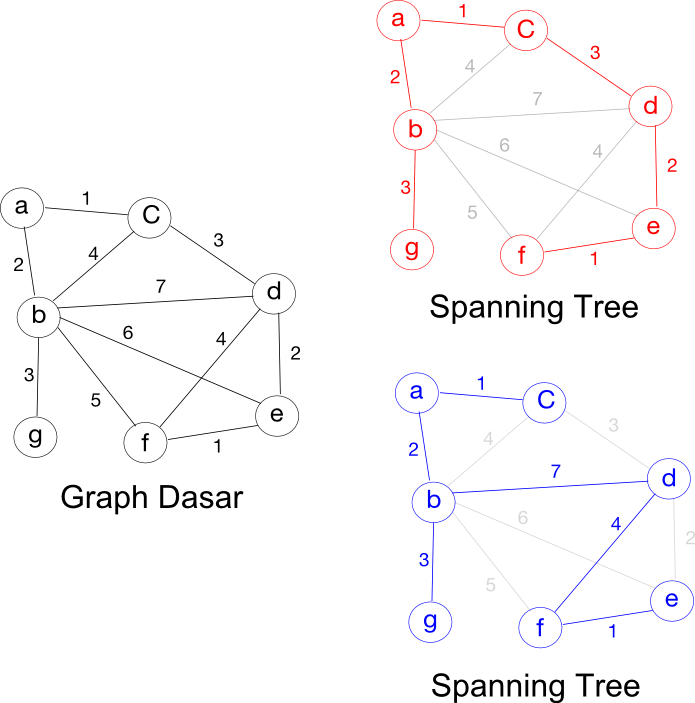
\includegraphics[width=\textwidth,keepaspectratio]{fig/SpanningTreeIntro.png}%
	\caption{Spanning Tree dalam sebuah Graph}%
	\label{fig:spanning-tree-intro}%
\end{figure}

Ketika menggambarkan sebuah Spanning Tree, kita dapat mengalokasikan nilai untuk setiap edge di dalamnya. Total bobot dari keseluruhan edge yang ada di dalam sebuah Spanning Tree kita kenal dengan istilah \textit{weight}. Sebuah Spanning Tree yang memiliki total nilai \textit{weight} terendah kita kenal dengan nama \textbf{Minimum Spanning Tree (MST)}.

MST memiliki banyak aplikasi pada perancangan sistem, terutama untuk sistem-sistem yang berhubungan dengan jaringan. Salah satu contoh pemanfaatan MST yaitu ketika sebuah perusahaan listrik ingin menambahkan jangkauan listrik ke suatu daerah, dengan memasang tiang listrik. Pemasangan tiang listrik pada suatu daerah akan dibatasi oleh berbagai batasan fisik, misalnya perusahaan listrik tidak mungkin memasang tiang listrik di dalam rumah penduduk. Jika kita mengasumsikan pemasangan hanya dilakukan pada sepanjang jalan, kita dapat membangun graph untuk merepresentasikan titik-titik yang dapat menjadi tempat pemasangan tiang listrik. Gambar~\ref{fig:electricity-installation} menggambarkan graph yang mungkin kita bangun untuk pemasangan listrik dalam sebuah kota.

\begin{figure}
    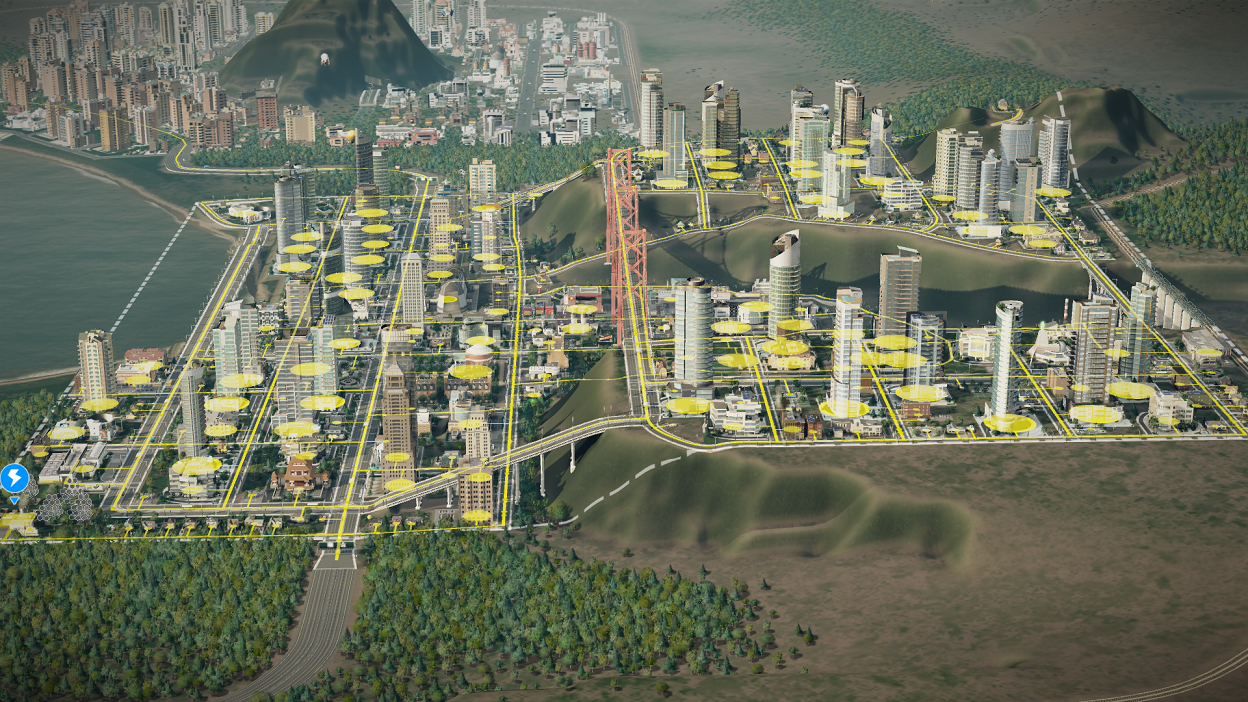
\includegraphics[width=\textwidth,keepaspectratio]{fig/ElectricityInstallation.png}%
	\caption{Jalur Pemasangan Tiang Listrik dalam Graph (Lingkaran Kuning adalah Vertex)}%
	\label{fig:electricity-installation}%
\end{figure}

Ketika sudah memiliki graph untuk jalur pemasangan tiang listrik seperti pada gambar~\ref{fig:electricity-installation}, kita kemudian dapat memberikan bobot kepada masing-masing edge yang ada. Acuan untuk nilai bobot yang digunakan dapat berbeda-beda, tergantung dari tujuan yang ingin dicapai. Contoh dari acuan yang dapat digunakan adalah jarak antar titik. Selain itu, kita juga dapat menggunakan biaya pemasangan sebagai tolak ukur bobot. Pemasangan tiang listrik pada sebuah bukit tentunya akan lebih mahal dan sulit, meskipun mungkin jarak yang ditempuh akan menjadi lebih sedikit.

Setelah memiliki graph pemasangan dan memilih acuan bobot dari edge, kita kemudian dapat mengguankan MST untuk menentukan jalur pemasangan listrik yang paling optimal. Metode pemanfaatan MST yang seperti ini dapat kita terapkan pada berbagai proses lain, seperti pemasangan kabel telepon, segmentasi gambar, dan lain-lain.

\section{Syarat dan Sifat MST}

Berdasarkan kajian singkat yang telah kita bahas pada bagian sebelumnya, terdapat beberapa kesimpulan yang dapat kita tarik. Pertama, sebelum membangun sebuah MST, kita terlebih dahulu harus memiliki dua hal berikut:

\begin{enumerate}
    \item Sebuah Graph satu arah
    \item Bobot dari masing-masing edge di dalam graph
\end{enumerate}

Kedua, sifat-sifat umum yang dimiliki oleh sebuah MST yaitu:

\begin{enumerate}
    \item Sebuah graph dapat memiliki banyak MST
    \item Jika setiap edge yang ada dalam graph memiliki nilai unik, maka hanya akan terdapat satu MST di dalam graph tersebut
    \item Jika bobot dari semua edge selalu bernilai positif, MST yang didapatkan akan selalu merupakan subgraph dengan bobot terkecil yang menghubungkan seluruh vertex
    \item Tidak boleh terdapat siklus (\textit(cycle)) di dalam MST, karena sebuah siklus karena total bobot graph dengan siklus akan selalu lebih besar dari graph tanpa siklus
\end{enumerate}

Pembentukan MST dari sebuah graph sendiri merupakan permasalahan optimasi yang dapat kita selesaikan dengan algoritma greedy. Pada bagian berikutnya kita akan membahas dua buah algoritma umum yang digunakan untuk membangun MST, yaitu algoritma Kruskal dan Prim.

\section{Algoritma Prim}

Algoritma Prim membangun sebuah MST dengan membuat tree dari sebuah graph terlebih dahulu. Tree yang akan dibangun oleh algoritma Prim dimulai dari sebuah vertex acak, yang nantinya akan dibangun satu demi satu vertex untuk menjadi MST. Gambar~\ref{fig:prims-proc} menunjukkan hubungan graph dengan pohon MST yang dibangun dengan algoritma Prim.

\begin{figure}
    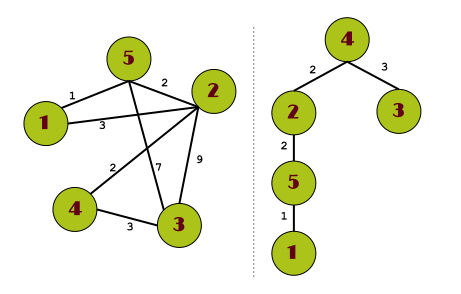
\includegraphics[width=\textwidth,keepaspectratio]{fig/PrimsProc.png}%
	\caption{Kiri: Graph Asal, Kanan: Tree MST dengan Prim; Sumber: http://architects.dzone.com/articles/algorithm-week-prims-minimum}%
	\label{fig:prims-proc}%
\end{figure}

Algoritma Prim membuat tree (selanjutnya disebut sebagai Spanning Tree) karena sebuah Tree tidak mungkin menghasilkan siklus dalam graph. Jika terdapat siklus di dalam graph yang dihasilkan, maka graph tersebut tidak dapat dikatakan sebagai sebuah MST.

Pembangunan Spanning Tree pada algoritma Prim sendiri dilakukan dalam beberapa tahap. Pada tahap pertama, kita menambahkan satu vertex sebagai akar dari Spanning Tree. Vertex manapun dapat dipilih sebagai akar dari Spanning Tree. Untuk iterasi-iterasi berikutnya, kita akan menambahkan vertex baru ke dalam Spanning Tree, sesuai dengan kriteria yang diwajibkan MST, yaitu vertex dengan bobot edge paling kecil dari vertex asal (sebelumnya).

Urutan pengambilan vertex untuk dimasukkan ke dalam Spanning Tree sendiri dapat dilakukan dengan beberapa cara. Misalnya, kita dapat mengambil vertex dengan edge terendah terhadap vertex terakhir di Spanning Tree dengan menandai tiap vertex dengan ukuran jarak. Pendekatan yang lebih pintar dapat memanfaatkan Priority Queue untuk menandai urutan prioritas vertex yang akan dikunjungi.

Agar tidak terlalu bingung, mari kita langsung lihat contoh implementasi algoritma Prim dengan Priority Queue. Fungsi Prim yang akan kita bangun menerima dua parameter, yaitu graph yang akan dicari MST-nya dan vertex awal untuk memulai algoritma Prim:

\lstinputlisting[language=Python, 
                 label={algo:prim-declaration},
                 firstline=3,
                 lastline=3,
                 caption=Deklarasi Fungsi Prim
                ]
                {code/16-prims-kruskal.py}

Selanjutnya, kita dapat menginisalisasi variabel-variabel awal yang akan kita butuhkan. Variabel pertama yang diinisialisasi adalah $vtx$, yang menyimpan semua vertex asal. $q$ merupakan Priority Queue yang akan menyimpan seluruh vertex beserta tingkat prioritasnya. Untuk menyederhanakan implementasi, Priority Queue akan kita simpan dalam sebuah Dictionary, dengan key berupa vertex dan value berupa nilai prioritas.

Sebagai nilai awal untuk $q$, kita akan mengisikan semua vertex yang ada, dengan prioritas maksimal (sebesar-besarnya). Hal ini dilakukan karena pada awal algoritma, kita belum mengetahui vertex mana yang akan dijalankan terlebih dahulu. Algoritma~\ref{algo:prim-init} menunjukkan langkah yang kita jalankan sejauh ini.

\lstinputlisting[language=Python, 
                 label={algo:prim-init},
                 firstline=4,
                 lastline=8,
                 caption=Deklarasi Variabel Awal Prim
                ]
                {code/16-prims-kruskal.py}

Selanjutnya, kita dapat membuat Spanning Tree yang akan dibangun, dalam variabel $t$. Sama seperti Priority Queue, kita akan menyimpan pohon di dalam Dictionary, dengan key sebagai nod yang aktif dan vertex sebagai orang tua (\textit{parent}) dari node tersebut. Pada node akar, kita akan mengisikan orang tua dengan nilai None.

Kita juga dapat sekaligus mengisikan nilai awal dari $t$ dan $q$, yaitu vertex awal yang dikirimkan oleh fungsi. Untuk $q$, prioritas vertex awal akan diisikan dengan $0$ agar pada iterasi selanjutnya kita dapat mulai dari vertex ini. Algoritma~\ref{algo:prim-init2} menunjukkan langkah kita sampai titik ini.

\lstinputlisting[language=Python, 
                 label={algo:prim-init2},
                 firstline=10,
                 lastline=13,
                 caption=Inisialisasi Nilai Awal Prim
                ]
                {code/16-prims-kruskal.py}

Iterasi pembangunan Spanning Tree dapat dilakukan dengan mengambil seluruh tetangga vertex dengan Prioritas Utama (nilai minimum), dan membandingkan bobot edge antara vertex asal dengan seluruh tetangganya. Kita mencari nilai bobot edge yang lebih kecil dari nilai prioritas di sini. Nilai edge terkecil ini diambil karena kita ingin mengambil nilai minimum. Jika edge lebih kecil dari prioritas, kita akan menjadikan nilai edge tersebut nilai prioritas vertex. Nilai prioritas vertex ini akan terus diperbaharui sampai vertex menjadi prioritas terkecil. Hal ini akan otomatis mengeliminasi siklus, karena edge siklus tidak akan dapat menjadi prioritas terkecil; ingat: edge siklus akan selalu lebih besar dari edge non-siklus.

Begitu kita mendapatkan edge dengan prioritas terkecil, kita dapat langsung memasukkannya ke dalam Spanning Tree. Algoritma~\ref{algo:prim-spanning-tree} menunjukkan langkah-langkah yang diambil untuk membangun Spanning Tree.

\lstinputlisting[language=Python, 
                 label={algo:prim-spanning-tree},
                 firstline=15,
                 lastline=25,
                 caption=Pembangunan Spanning Tree
                ]
                {code/16-prims-kruskal.py}

Setelah mendapatkan Spanning Tree dari algoritma Prim, kita dapat membangun Graph MST-nya dengan cukup mudah: telusuri tree dan bangun node serta edge-nya, seperti yang dilakukan pada Algoritma~\ref{algo:prim-mst}.

\lstinputlisting[language=Python, 
                 label={algo:prim-mst},
                 firstline=1,
                 lastline=33,
                 caption=Pembangunan MST dari Spanning Tree
                ]
                {code/16-prims-kruskal.py}

Keseluruhan algoritma Prim yang kita bangun dapat dilihat pada Algoritma~\ref{algo:prim-complete}.

\lstinputlisting[language=Python, 
                 label={algo:prim-complete},
                 caption=Algoritma Prim
                ]
                {code/16-prims-kruskal.py}


\section{Algoritma Kruskal}

Algoritma Kruskal membangun sebuah MST dengan mengurutkan semua edge yang ada di dalam sebuah graph, dari mulai beban yang terkecil hingga terbesar. Edge yang telah terurut ini kemudian dimasukkan satu per satu ke dalam MST, dengan tetap memperhatikan apakah sebuah siklus terjadi atau tidak. Langkah ini diulangi sampai didapatkan semua vertex di dalam MST.

Secara terstruktur, langkah-langkah untuk algoritma Kruskal adalah sebagai berikut:

\begin{enumerate}
    \item Urutkan semua edge secara menaik, berdasarkan bobot edge.
    \item Ambil edge terkecil. Cek apakah edge membentuk siklus dari MST yang telah terbentuk. Jika tidak, masukkan edge ini ke dalam MST. Jika ya, jangan masukkan.
    \item Ulangi langkah kedua sampai jumlah edge dalam MST adalah jumlah vertex - 1
\end{enumerate}

Langkah terakhir, tentunya dapat juga diganti dengan mengecek sampai keseluruhan edge habis, yang akan sedikit lebih menyederhanakan algoritma dengan mengorbankan jumlah langkah eksekusi.

\subsection{Cek Siklus pada Graph}

Deteksi apakah sebuah edge baru membentuk siklus di dalam MST dapat dilakukan dengan banyak algoritma. Salah satu algoritma yang paling populer yaitu algoritma Union-Find. Algoritma Union-Find diimplementasikan pada struktur data \textbf{Disjoint Set} dan dapat digunakan untuk berbagai keperluan. Pada bagian ini, kita akan menggunakan Union-Find untuk melakukan pengecekan apakah sebuah graph memiliki siklus atau tidak.

Dasar dari algoritma Union-Find yaitu dua buah operasi, Union dan Find:

\begin{itemize}
    \item \textbf{\textit{Union}} menggabungkan dua buah subset menjadi satu subset baru.
    \item \textbf{\textit{Find}} merupakan operasi untuk menentukan di dalam subset manakah sebuah elemen berada.
\end{itemize}

Implementasi sederhana dari Union dan Find dapat dilihat pada Algoritma~\ref{algo:union-find}.

\lstinputlisting[language=Python, 
                 label={algo:union-find},
                 firstline=36,
                 lastline=57,
                 caption=Implementasi Union dan Find
                ]
                {code/16-prims-kruskal.py}

Untuk mencari sebuah siklus di dalam graph, kita dapat menggunakan kedua operasi di atas dengan langkah berikut untuk mendeteksi siklus:

\begin{enumerate}
    \item Masukkan semua vertex yang ada ke dalam sebuah subset. \textit{Parent} dari masing-masing vertex adalah dirinya sendiri, karena kita belum membangun subset dengan lengkap. Kita kemudian dapat memberikan tingkat dari setiap vertex, dimulai dari 0. Tingkatan ini nantinya akan menentukan posisi akhir vertex di dalam subset.
    \item Ambil satu edge dengan bobot terendah, dan telusuri \textit{Parent} dari kedua buah vertex yang membentuk edge tersebut. Jika parent sama, maka kedua edge berada dalam subset yang sama. Hal ini berarti graph memiliki siklus. Jika parent berbeda, lakukan union terhadap kedua graph.
    \item Ulangi langkah kedua sampai seluruh edge telah dioperasikan.
\end{enumerate}

Algoritma~\ref{algo:cycle-detection} memperlihatkan contoh implementasi pendeteksian siklus pada sebuah graph, sesuai dengan langkah-langkah yang telah dijabarkan di atas.

\lstinputlisting[language=Python, 
                 label={algo:cycle-detection},
                 firstline=59,
                 lastline=68,
                 caption=Deteksi Siklus dalam Graph
                ]
                {code/16-prims-kruskal.py}

Kita kemudian dapat melihat bagaimana edge yang bukan siklus (pada baris ke 10 di algoritma~\ref{algo:cycle-detection} dapat langsung dijadikan sebagai anak pohon MST dalam algoritma Kruskal. Hal ini menyebabkan implementasi algoritma Kruskal tidak berbeda jauh dari algoritma~\ref{algo:cycle-detection}. 

\subsection{Kruskal}

Dari apa yang telah kita dapatkan, kita kemudian dapat mengimplementasikan algoritma Kruskal seperti yang dapat dilihat pada algoritma~\ref{algo:kruskal-core}.

\lstinputlisting[language=Python, 
                 label={algo:kruskal-core},
                 firstline=59,
                 lastline=69,
                 caption=Deteksi Siklus dalam Graph
                ]
                {code/16-prims-kruskal.py}

Jika dilengkapi dengan implementasi Disjoint Set dan Union-Find maka implementasi lengkap algoritma Kruskal dapat dilihat pada algoritma~\ref{algo:kruskal-all}.

\lstinputlisting[language=Python, 
                 label={algo:kruskal-all},
                 firstline=35,
                 lastline=71,
                 caption=Algoritma Kruskal Lengkap
                ]
                {code/16-prims-kruskal.py}
